\documentclass[10pt, twocolumn, a4paper]{article}

% Additional packages.
    \usepackage{graphicx}  % Images.
    \usepackage{esint}  % Additional integral symbols (eg: \iint).
    \usepackage[T1]{fontenc}  % Additional symbols (eg: \eth).
    \usepackage{multicol}
    \usepackage{float}
    \usepackage{hyperref}

% Margins.
    \usepackage[top=1cm, bottom=1.5cm, left=1cm, right=1cm]{geometry}
    \setlength{\columnsep}{1cm}
    \raggedbottom

% Space between paragraphs.
    \usepackage{parskip}
    % \setlength{\parskip}{11pt}

% Block break and word break.
    \hbadness=10000
    % \emergencystretch=\maxdimen
    % \hyphenpenalty=10000
    % \tolerance=1zz

% Title.
    \begin{document}
    \title{Finger sensing surrounding physical buttons}
    \author{
        Author: Marcos Díaz\\
        Research period: 2021, 2022\\
        Publication: November 2022
    }
    \date{}
    \maketitle

% Body.

\begin{abstract}
    By adding finger sensing capabilities such as touch-sensitive surfaces or proximity sensors surrounding physical buttons (push-down switches), it is possible to improve the functionality of these buttons with minimal increase in complexity of use; without the tradeoffs of virtual buttons, nor requiring the user to move the fingers to different locations nor to use multiple fingers.
\end{abstract}

\section*{Acronyms / Glossary}
    {\textbf{ABXY}}: Face buttons in a standard videogame controller.\\
    {\textbf{FPS}}: First Person Shooter.\\
    {\textbf{HID}}: Human Interface Device.\\
    {\textbf{USB}}: Universal Serial Bus.\\
    {\textbf{VR}}: Virtual Reality.

\section{Introduction}
    Complexity in input devices such as computer mouse and videogame controllers (including \textbf{VR} controllers) have been increasing over the years, featuring many novel input methods such as touch-sensitive surfaces \cite{capacitative}, pressure sensors \cite{pressure}, motion sensors \cite{piezo_mems}, and even biometric sensors \cite{biometrics}. But also getting a significant increase in the number of physical momentary switch buttons and analog input axis.

    \begin{table}[H]
        \centering
        \small
        \caption{Mouse input complexity over time}
        \vspace{2mm}
        \begin{tabular}{|r|r|r|}
            \hline
                Year & Mouse & Buttons \\
            \hline
                1981 & Xerox Star (mouse) & 2 \\
                1990 & Logitech MouseMan & 3 \\
                2005 & Logitech G3 & 6 \\
                2009 & Razer Naga & 16 \\
                2012 & Logitech G600 & 20 \\
            \hline
        \end{tabular}
    \end{table}

    \vspace{-5mm}
    \begin{table}[H]
        \centering
        \small
        \caption{Gamepad input complexity over time}
        \vspace{2mm}
        \begin{tabular}{|r|r|r|r|}
            \hline
                Year & Gamepad & Buttons & Analog \\
                     &         &         & axis \\
            \hline
                1983 & Nintendo NES & 8 & 0 \\
                1995 & PlayStation 1 & 14 & 0 \\
                2000 & PlayStation 2 (DualShock 2) & 16 & 4 \\
                2001 & Nintendo GameCube & 12 & 6 \\
                2017 & Nintendo Switch (Pro) & 18 & 10 \\
                2022 & PlayStation 5 (DualSense Edge) & 17 & 14 \\
            \hline
        \end{tabular}
    \end{table}

    % Such increase in input complexity goes in parallel with the increase in complexity in computer applications and videogames and the videogame industry becoming mainstream.

\pagebreak
\section{Problem}
    With the increase of input complexity, placement of so many buttons/surfaces/sensors on the devices while maintaining usability and accessibility, became very challenging.

    For example in a videogame gamepad with classic layout (eg. Xbox controller), both the \textbf{ABXY} face buttons and the right thumbstick are expected to be operated with the same finger (right thumb), this creates a limitation on the actions that can be performed simultaneously, for example in the most common \textbf{FPS} control layout is not possible to aim (right thumbstick) while jumping (A button).

    A common solution to pack more controls into a reduced space is to combine several input methods of different nature, for example adding physical momentary buttons underneath other kind of controls, such as in clickable mouse scrollwheel, clickable thumbstick, or clickable trackpad. In the case of trackpad, instead of featuring separate buttons next to it to perform primary and secondary clicks, adding a physical momentary button under the touch-sensitive surface provides feedback to trackpad clicks in a convenient way without forcing the user to move the finger to another location nor to use another finger.

    \subsection{Problem with virtual buttons}
        Clickable trackpads became very popular, and they are featured not only in most laptops, but also in videogame controllers such as Sony DualShock 4 (2013), and Steam Controller (2015). But all these share a common issue: when emulating multiple buttons by determining finger location on the trackpad (2 mouse buttons in a laptop trackpad, or ABXY buttons in Steam Controller right trackpad), users do not have physical feedback about which one of the virtual buttons have been pressed, so they do not know if they pressed with the correct finger placement until after the button input has been sent. For example in the case of pressing in-between virtual buttons, the firmware/software governing the devices can decide either to assume both virtual buttons were pressed, or neither of them were pressed, but both of these approaches are problematic.

        Additionally, virtual buttons have the limitation of not being able to press/release several (virtual) buttons in arbitrary combinations. For example in a trackpad in which single click emulates mouse primary button and 2-finger click emulates secondary mouse button, is not possible to virtually press primary and secondary mouse buttons at the same time. Similarly when the Steam Controller right trackpad emulates ABXY buttons, is not possible for example to press and hold (A) then press (B) with an additional "click" feedback, since the physical button underneath the touch surface is already depressed.


\section{Finger-sensing surrounding\\physical buttons}
\label{solution_1}
    Instead of trying to make touch-sensitive surfaces clickable, a different approach is to add finger-sensing properties (touch surfaces or proximity sensors) surrounding physical momentary switch buttons as they are.

    In the case of a videogame controller, the surface between and/or around the ABXY buttons can be touch-sensitive, allowing the user to drag the finger on the touch-sensitive surface while with the same finger (usually right thumb) operating the ABXY buttons when required. This way there are no tradeoffs in button press/release feedback, possible button combinations to be pressed, nor ambiguity about the button location.

    The adjacent placement of the buttons to the touch-sensitive surface allows both to be operated simultaneously, in the case of (A) and (B) reaching the center (touch surface) with the fingertip and pressing the button with the base of the distal phalanx; or in the case of (X) and (Y) buttons pressing the button with the fingertip and touching the center surface with the base of the distal phalanx.

    While it would be possible to feature a full operative trackpad (for mouse control) in-between the buttons, arguably the small surface area would be better suited for emulating a vertical and/or horizontal mouse scroll wheel with directional swipes, or just to detect that a finger is resting in-between the ABXY buttons.

    Figure \ref{fig_1} shows a videogame controller with a touch-sensitive surface embedded in-between the typical (momentary switch) ABXY buttons. The size of the surface could be significantly larger (completely surrounding all the buttons) or significantly smaller, though a small surface would limit the potential functionality. This touch-sensitive surface could determine the finger position by using capacitive sensing \cite{capacitative}, or just detect if the finger is resting on it with a simple (single resistor) capacitance measurement.
    \begin{figure}[H]
        \begin{center}
            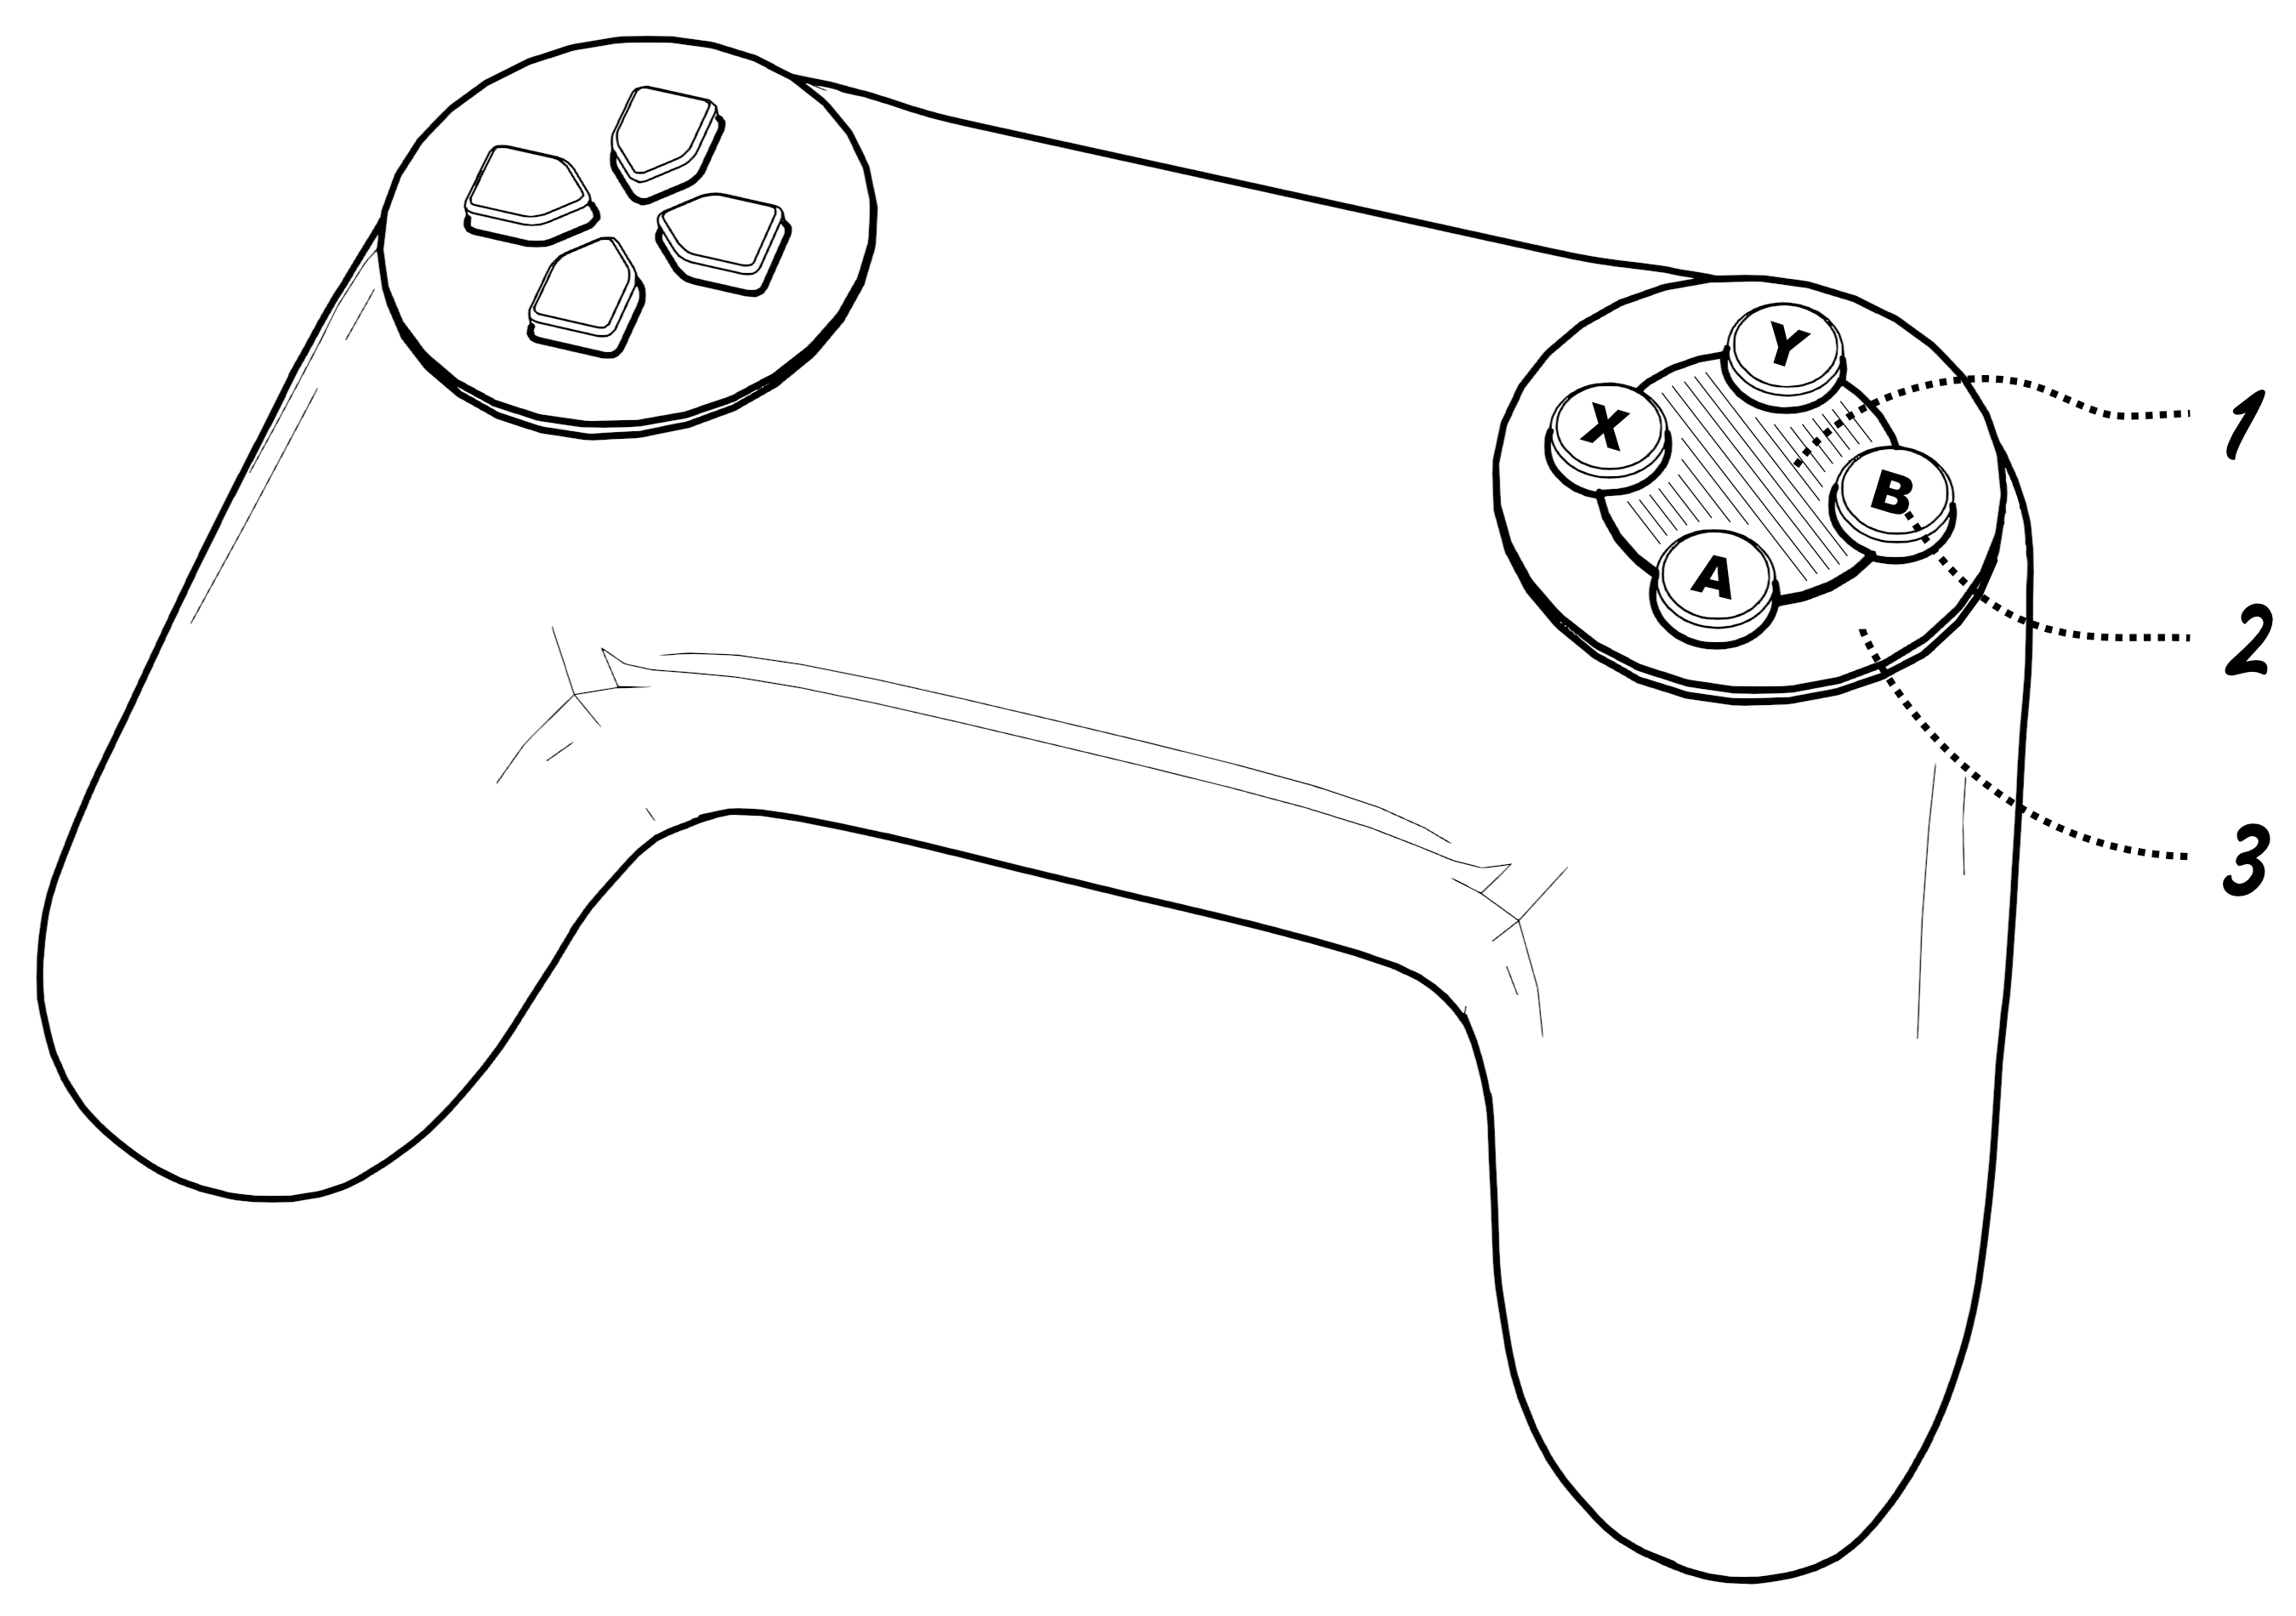
\includegraphics[width=0.9\linewidth]{figure_A1.png}
            \caption{Touch-sensitive surface surrounding buttons\\}
            \label{fig_1}
            \small
                \vspace{2mm}
                (1): Touch-sensitive surface.\\
                (2): Push-down momentary switches/buttons.\\
                (3): Non-touch-sensitive enclosure of the controller.
        \end{center}
    \end{figure}

    \pagebreak
    Figure \ref{fig_2} shows a videogame controller with a proximity sensor underneath the central position in-between the typical (momentary switch) ABXY buttons. The proximity sensor detect if the finger is resting in-between the buttons. Any kind of proximity sensor could be fit for this purpose, including infrared \cite{infrared}, ultrasonic \cite{ultrasonic}, or even a low resolution camera.
    \begin{figure}[H]
        \begin{center}
            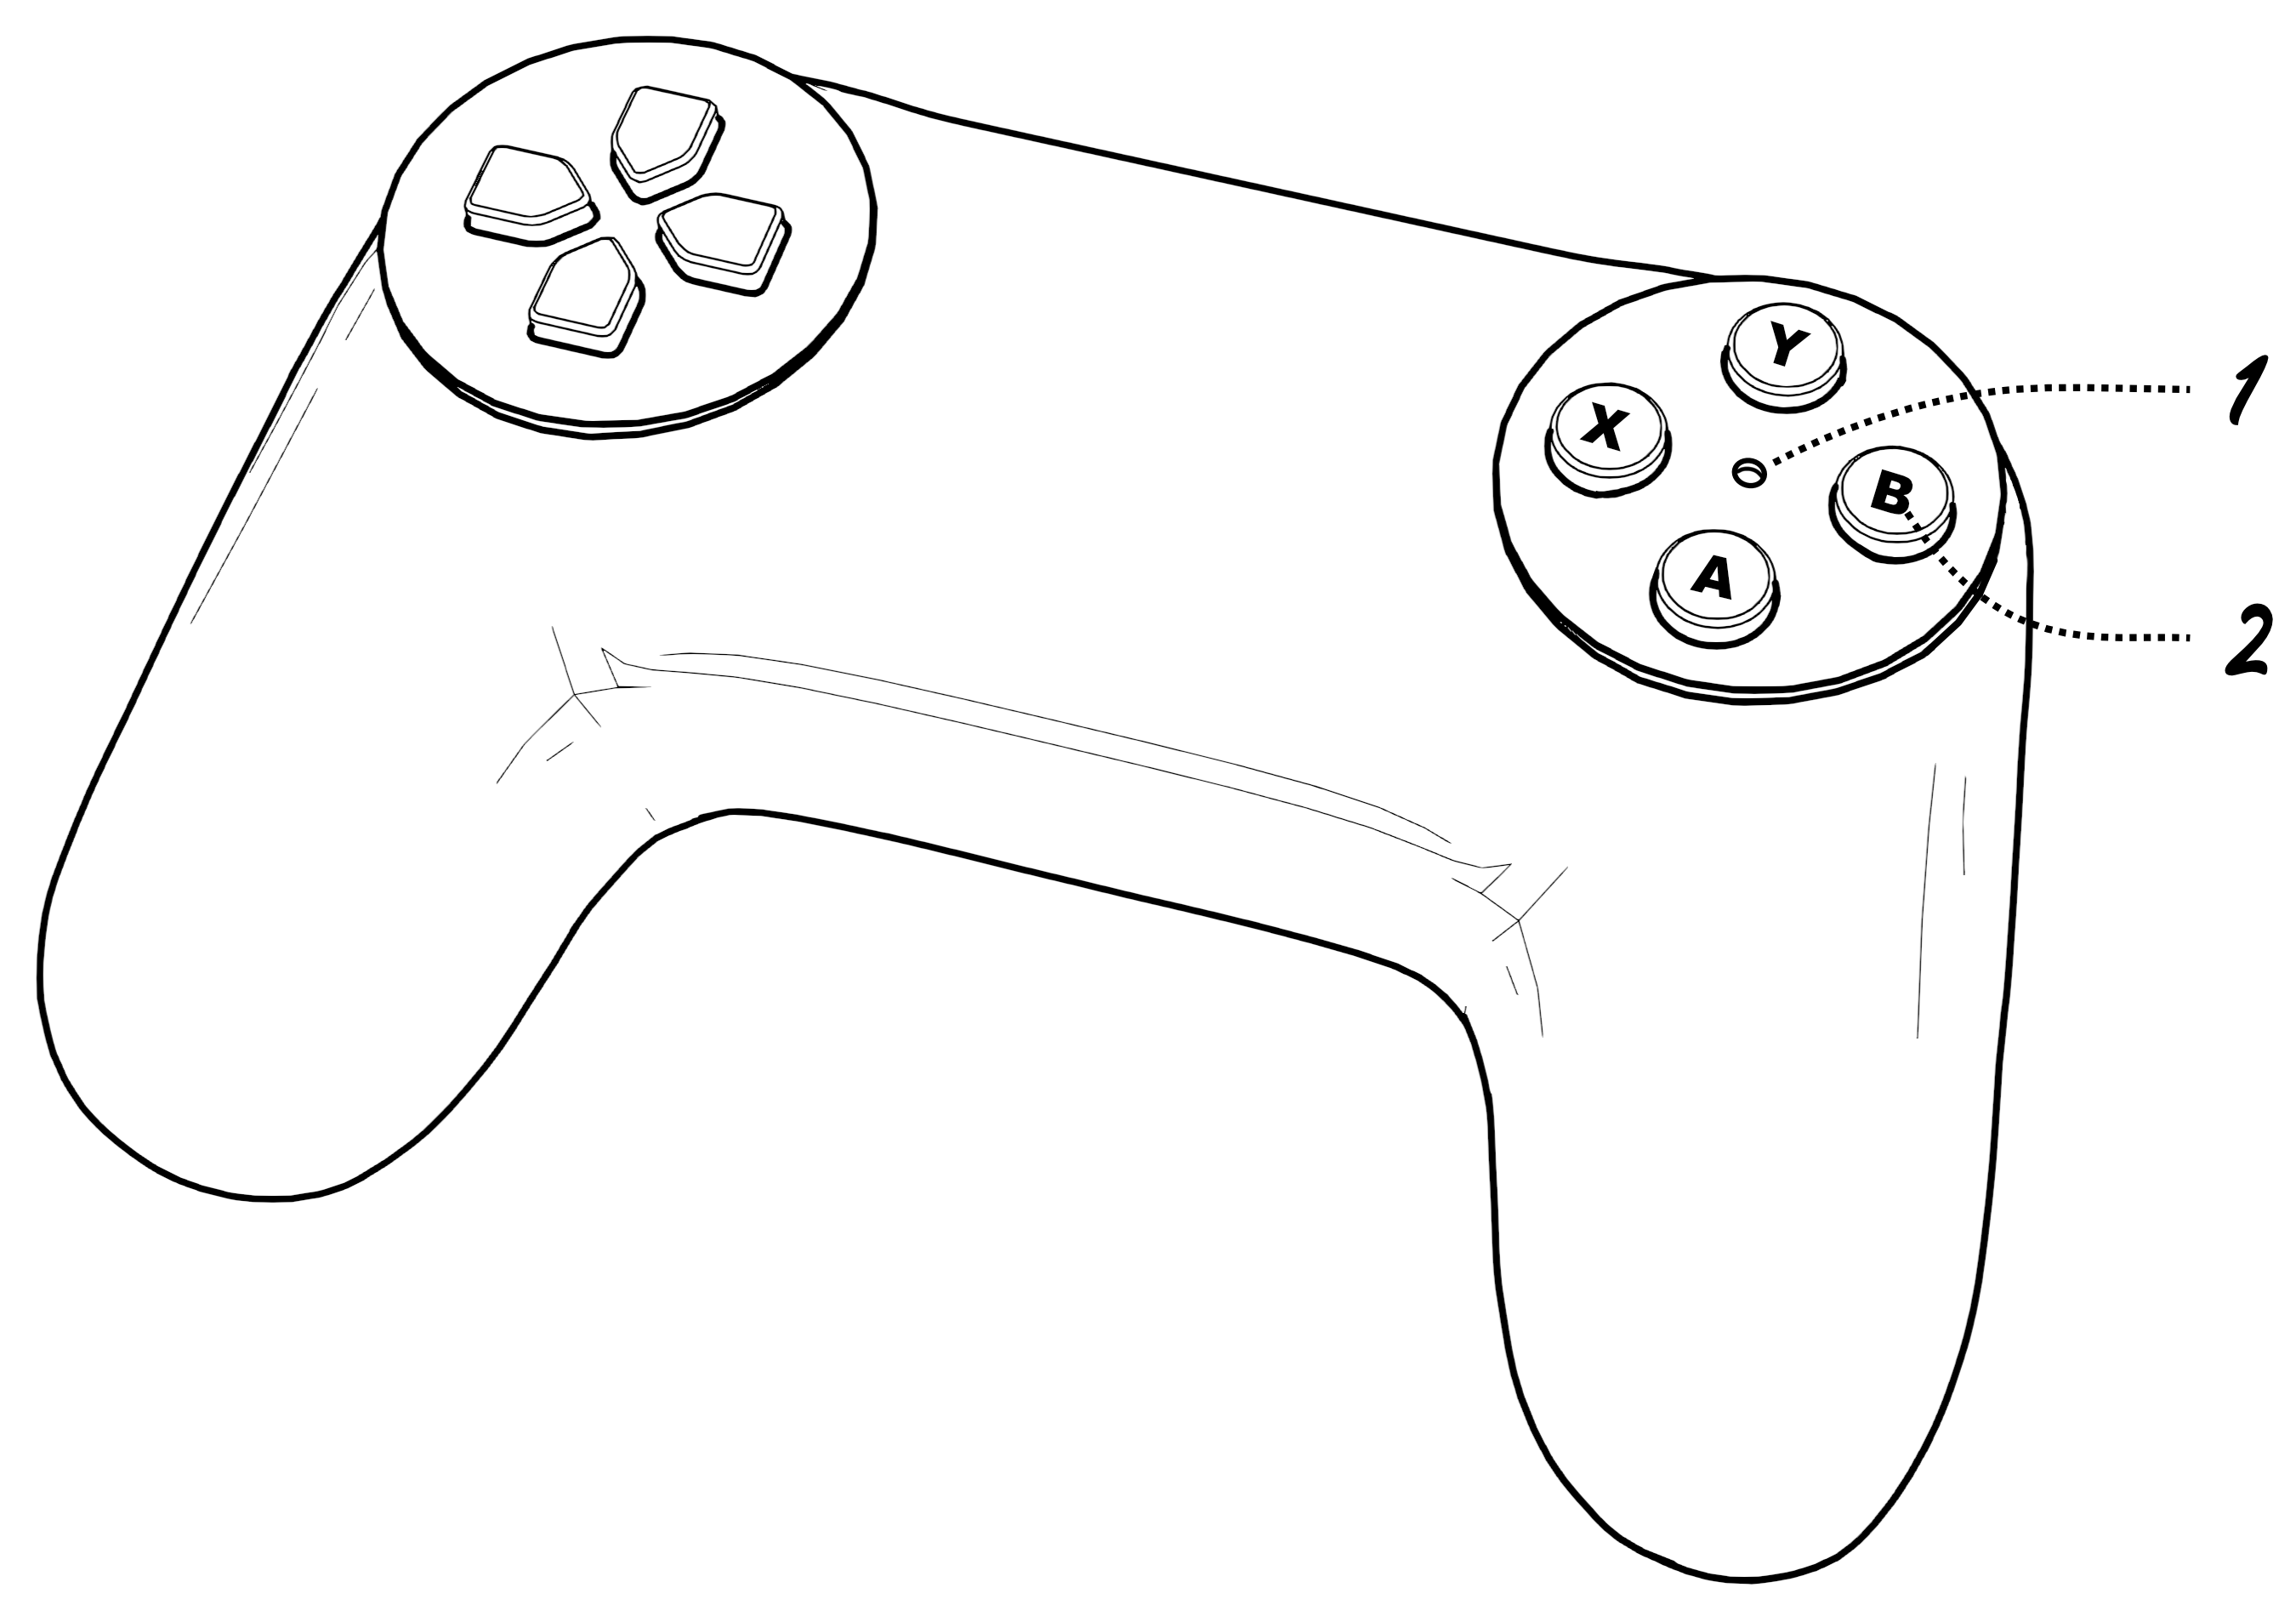
\includegraphics[width=0.9\linewidth]{figure_A2.png}
            \caption{Proximity sensor in-between buttons\\}
            \label{fig_2}
            \small
                \vspace{2mm}
                (1): Proximity sensor aperture.\\
                (2): Push-down momentary switches/buttons.
        \end{center}
    \end{figure}

\section{Finger-sensing on physical\\buttons}
    Alternatively the button themselves could feature finger-sensing capabilities.

    While this solution is very constrained in available space, and could not feature a functional trackpad, binary touch sensing (touching / not-touching) is enough to increase the functionality of the button. Additionally some proximity sensors are capable of determining distance, and therefore analog values for how close the finger is to the button could be used as input data.

    Figure \ref{fig_B1} shows a momentary switch with an electrically conductive button (or button cap) that allows for simple capacitance measurement. With this solution the button itself goes from 2 possible states (released, pressed) to 3 possible states (released-not-touched, released-touched, pressed).
    \begin{figure}[H]
        \begin{center}
            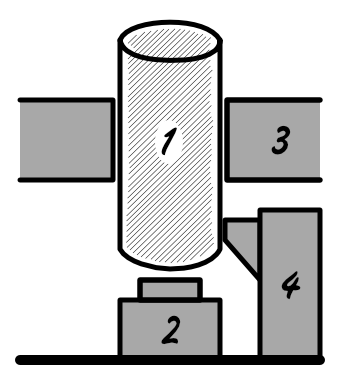
\includegraphics[width=0.4\linewidth]{figure_B1.png}
            \caption{Touch-sensitive button\\}
            \label{fig_B1}
            \small
                \vspace{2mm}
                (1): Electrically conductive button.\\
                (2): Push-down momentary switch.\\
                (3): Device external case.\\
                (4): Connector with bending blade/shrapnel.
        \end{center}
    \end{figure}

    \pagebreak
    Figure \ref{fig_B2} shows a momentary switch with an electrically conductive button, but the only the button cap and the button base (making contact with the connector) are conductive, while the central part is not conductive, so it is independent from a touch surface surrounding the buttons as defined in section \ref{solution_1}.
    \begin{figure}[H]
        \begin{center}
            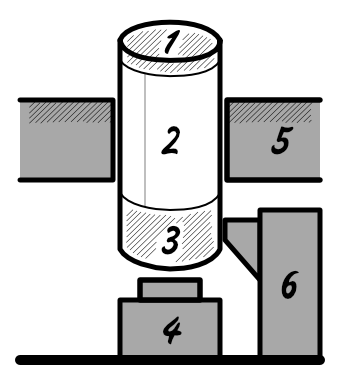
\includegraphics[width=0.4\linewidth]{figure_B2.png}
            \caption{Touch-sensitive button cap\\}
            \label{fig_B2}
            \small
                \vspace{2mm}
                (1): Electrically conductive button cap.\\
                (2): Non-conductive button center.\\
                (3): Conductive button base (connected with the cap).\\
                (4): Push-down momentary switch.\\
                (5): Device external case with touch-sensitive surface.\\
                (6): Connector with bending blade/shrapnel.
        \end{center}
    \end{figure}

    Figure \ref{fig_B3} shows a button with an embedded proximity sensor facing upwards, also allowing for 3 possible states (released-not-touched, released-touched, pressed), or additionally providing analog values for how close the finger is to the button.
    \begin{figure}[H]
        \begin{center}
            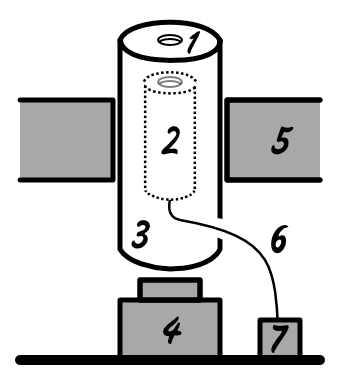
\includegraphics[width=0.4\linewidth]{figure_B3.png}
            \caption{Button with proximity sensor\\}
            \label{fig_B3}
            \small
                \vspace{2mm}
                (1): Aperture on the button cap.\\
                (2): Proximity sensor.\\
                (3): Button hosting the proximity sensor.\\
                (4): Push-down momentary switch.\\
                (5): Device external case.\\
                (6): Proximity sensor cable.\\
                (7): Connector for the proximity sensor cable.
        \end{center}
    \end{figure}

\section{Methodology}
    The hypothesis about how to employ touch-sensing capabilities around physical buttons were originally tested with breadboard prototypes using a Raspberry Pi Pico being used as \textbf{USB} \textbf{HID} (computer input device), common momentary switches (AlpsAlpine SKHHAJA010), and a metal sheet in-between the buttons acting as a simple touch-sensitive surface by measuring capacitance timing.

    Later more advanced test devices were created with a 3D printer, buttons with longer travel, and electrically conductive filament for more complex capacitative surfaces.

\pagebreak
\section{Potential applications}
    While this research is focused in videogame input and ABXY buttons of standard layout gamepad, the same principles can be applied to the other buttons on a gamepad, or any other kind of videogame controller, including VR handheld controllers, or even generalist computer input devices such as computer mouse or keyboard.

    The implementation for detecting if a finger is resting or close to physical buttons, while simple, can be very effective in engaging/disengaging additional features on a controller, as for example \textbf{IMU}-based motion and/or rotation, without requiring the user to operate additional buttons nor to dedicate a finger exclusively for it.

    Alternative applications in which fast and responsive controls are necessary while keeping a simple interface may also be a good fit, as for example medical machinery, music equipment, or drone control.

\begin{thebibliography}{99}
    \bibitem{capacitative}
        Puers, Robert.
        "Capacitive sensors: when and how to use them"
        Sensors and Actuators A: Physical 37.
        (1993).
        \url{https://doi.org/10.1016/0924-4247(93)80019-D}
    \bibitem{pressure}
        Lim, Hee C., Brian Schulkin, M. J. Pulickal, Sheng Liu, R. Petrova, G. Thomas, S. Wagner, K. Sidhu, and John F.
        "Flexible membrane pressure sensor"
        Sensors and Actuators A: Physical 119.2.
        (2005).
        \url{https://doi.org/10.1016/j.sna.2004.10.012}
    \bibitem{piezo_mems}
        Tadigadapa, S. A. K. M., and K. Mateti.
        "Piezoelectric MEMS sensors: state-of-the-art and perspectives"
        Measurement Science and technology.
        (2009).
        \url{https://doi.org/10.1088/0957-0233/20/9/092001}
    \bibitem{biometrics}
        Mirza-Babaei, P., Nacke, L. E., Gregory, J., Collins, N., Fitzpatrick, G.
        "How does it play better? exploring user testing and biometric storyboards in games user research".
        (2013).
        \url{https://doi.org/10.1145/2470654.2466200}
    \bibitem{ultrasonic}
        Canali, C., De Cicco, G., Morten, B., Prudenziati, M., Taroni, A.
        "A temperature compensated ultrasonic sensor operating in air for distance and proximity measurements".
        IEEE Transactions on Industrial electronics, (4).
        (1982).
        \url{https://doi.org/10.1109/TIE.1982.356688}
    \bibitem{infrared}
        Johnston, Alan R.
        "Proximity sensor technology for manipulator end effectors"
        Mechanism and Machine Theory 12.1.
        (1977).
        \url{https://doi.org/10.1016/0094-114X(77)90061-1}
\end{thebibliography}

% \section*{Special thanks to}
% \vspace{-2mm}
%     X Y

\end{document}




